%%%%%%%%%%%%%%%%%%%%%%%%%%%%%%%%%%%%%%%%%
% Large Colored Title Article
% LaTeX Template
% Version 1.1 (25/11/12)
%
% This template has been downloaded from:
% http://www.LaTeXTemplates.com
%
% Original author:
% Frits Wenneker (http://www.howtotex.com)
%
% License:
% CC BY-NC-SA 3.0 (http://creativecommons.org/licenses/by-nc-sa/3.0/)
%
%%%%%%%%%%%%%%%%%%%%%%%%%%%%%%%%%%%%%%%%%

%----------------------------------------------------------------------------------------
%	PACKAGES AND OTHER DOCUMENT CONFIGURATIONS
%----------------------------------------------------------------------------------------

\documentclass[DIV=calc, paper=letter, fontsize=10pt, twocolumn]{scrartcl}	 % A4 paper and 11pt font size

\usepackage{graphicx}
\usepackage{hyperref}
\usepackage{lipsum} % Used for inserting dummy 'Lorem ipsum' text into the template
\usepackage[english]{babel} % English language/hyphenation
\usepackage[protrusion=true,expansion=true]{microtype} % Better typography
\usepackage{amsmath,amsfonts,amsthm} % Math packages
\usepackage[svgnames]{xcolor} % Enabling colors by their 'svgnames'
\usepackage[hang, small,labelfont=bf,up,textfont=it,up]{caption} % Custom captions under/above floats in tables or figures
\usepackage{booktabs} % Horizontal rules in tables
\usepackage{fix-cm}	 % Custom font sizes - used for the initial letter in the document
\usepackage{booktabs}
\usepackage{paralist}

\usepackage{sectsty} % Enables custom section titles
\allsectionsfont{\usefont{OT1}{phv}{b}{n}} % Change the font of all section commands

\usepackage{fancyhdr} % Needed to define custom headers/footers
\pagestyle{fancy} % Enables the custom headers/footers
\usepackage{lastpage} % Used to determine the number of pages in the document (for "Page X of Total")

% Headers - all currently empty
\lhead{}
\chead{}
\rhead{}

% Footers
\lfoot{}
\cfoot{}
\rfoot{\footnotesize Page \thepage\ of \pageref{LastPage}} % "Page 1 of 2"

\renewcommand{\headrulewidth}{0.0pt} % No header rule
\renewcommand{\footrulewidth}{0.4pt} % Thin footer rule

\usepackage{lettrine} % Package to accentuate the first letter of the text
\newcommand{\initial}[1]{ % Defines the command and style for the first letter
\lettrine[lines=3,lhang=0.3,nindent=0em]{
\color{DarkGoldenrod}
{\textsf{#1}}}{}}

%----------------------------------------------------------------------------------------
%	TITLE SECTION
%----------------------------------------------------------------------------------------

\usepackage{titling} % Allows custom title configuration

\newcommand{\HorRule}{\color{DarkGoldenrod} \rule{\linewidth}{1pt}} % Defines the gold horizontal rule around the title

\pretitle{\vspace{-30pt} \begin{flushleft} \HorRule \fontsize{50}{50} \usefont{OT1}{phv}{b}{n} \color{DarkRed} \selectfont} % Horizontal rule before the title

\title{\Huge Literature Search Made Easy: Mining Online Archives for Research Topic Trends} % Your article title

\posttitle{\par\end{flushleft}\vskip 0.5em} % Whitespace under the title

\preauthor{\begin{flushleft}\large \lineskip 0.5em \usefont{OT1}{phv}{b}{sl} \color{DarkRed}} % Author font configuration

\author{Bo Wang, Min Liu } % Your name

\postauthor{\footnotesize \usefont{OT1}{phv}{m}{sl} \color{Black} % Configuration for the institution name
Stanford University % Your institution

\par\end{flushleft}\HorRule} % Horizontal rule after the title

\date{} % Add a date here if you would like one to appear underneath the title block

%----------------------------------------------------------------------------------------

\begin{document}

\maketitle % Print the title

\thispagestyle{fancy} % Enabling the custom headers/footers for the first page 

%----------------------------------------------------------------------------------------
%	ABSTRACT
%----------------------------------------------------------------------------------------

% The first character should be within \initial{}
\initial{M}\textbf{any of us have been faced with this situation: we found a certain field of research intriguing, went to an online archive to search for related papers, and the results were just less than satisfactory: they are too unstructured to obtain a big picture, such as how this field evolves over time, what sub-fields it is composed of, and which papers are most influential. Instead of relying on human instinct for such insights, our project provides an alternative: using machine learning algorithms to peruse thru online archives, generate information of interest, and present them in a human friendly way. Common topic modeling algorithms like latent Dirichlet allocation (LDA) do a good job in clustering topics, however, they are not able to extract key phrases in the corpus. We found phrase extraction an indispensable enabler towards a useful research trend analysis system, since many research topics are formed by multiple words. Only using individual terms is too abstract for a newcomer to a field to figure out the context. To solve this problem, we designed a mechanism to extract phrases in documents and then integrated it into hierarchical latent Dirichlet allocation (hLDA) and dynamic topic model (DTM) to automatically generate topic hierarchy and topic trends. In our experiments with 14185 condensed matter physics papers from arXiv, our method effectively classified papers into a tree of topics with significant meaning and picked out most representative words and phrases of each topic. With phrases, the result is visibly better than those purely relying on individual terms.}

%----------------------------------------------------------------------------------------
%	ARTICLE CONTENTS
%----------------------------------------------------------------------------------------


\section*{Background}

\subsection*{Latent Dirichlet Allocation (LDA)}
Latent Dirichlet Allocation (LDA) \cite{1} is a Bayesian generative probabilistic model of a corpus. It assumes that documents are random mixtures of latent topics, where each topic is characterized by a distribution over words. Here we describe the smoothed LDA since this is the version of LDA that serves as the basis of the other models used in this paper.
Smoothed LDA assumes the following generative process (Figure ~\ref{fig: LDA}) for a document in a corpus D:
\begin{enumerate}
  \item Choose $N \sim Poisson(\xi)$.
  \item Choose $\theta \sim Dir(\alpha)$.
  \item Choose $\beta \sim Dir(\eta)$.
  \item For each of the N words $w_n$:
  	\begin{enumerate}
  	  	\item Choose a topic $z_n \sim  Multinomial(\theta)$
    		\item Choose a word $w_n$ from $p(w_n|z_n, \beta)$, a multinomial probability conditioned on the topic $z_n$.
  	\end{enumerate}
\end{enumerate}
The key computational problem of LDA is to infer the hidden variables, i.e. finding what hidden topic structure is most likely to generate the observed corpus with the above generative process. Once the posterior of the hidden variables are computed, it can be used to output topics words that appear most often in each topic. Details of the algorithm can be found in \cite{1}.
			\begin{figure}[!ht]
				\centerline{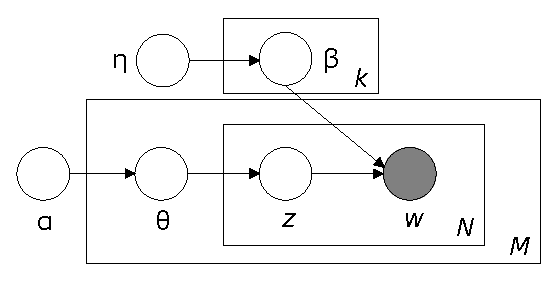
\includegraphics[scale = 0.8]{BleiNgJordan2003.eps}}
				\caption{Illustration of generative process of LDA \cite{1}}
				\label{fig: LDA}
			\end{figure}

\subsection*{Hierarchical Latent Dirichlet Allocation (hLDA)}
Hierarchical Latent Dirichlet Allocation (hLDA) \cite{2} is an extension of LDA which analyzes hierarchies of topics in a corpus. Instead of constraining each document to have a fixed finite number of k topics as LDA does, it allows an infinite number of topics, which are organized in a hierarchy, with the most abstract topics near the root of the hierarchy and more concrete topics near the leaves. In hLDA, a word is generated not based on the topic but a path of topics (from the root topic to the leaf topic) it belongs to.\newline
The generative process (Figure ~\ref{fig: hLDA})can be illustrated as:
\begin{enumerate}
  \item Let $c_1$ be the root topic.
  \item For each level $l \in 2,\ldots, L$ :
  	\begin{enumerate}
		\item Draw a sub-topic from topic $c_{l - 1}$.
		\item Set $c_l$ to be that sub-topic.
	\end{enumerate}

  \item Draw an L dimensional topic proportion vector $\theta$ from $Dir(\alpha)$.
  \item For each word $n \in \{ 1, \ldots, N \}$:
  	\begin{enumerate}
  	  	\item Draw $z \in \{ 1, \ldots, L \}$ from {\it Multinomial($\theta$)}.
    		\item Draw $w_n$ from the topic associated with $c_z$.
  	\end{enumerate}
\end{enumerate}
,where the root topic is the topic on level 1, its sub-topics are those on level 2, etc.
			\begin{figure}[!ht]
				\centerline{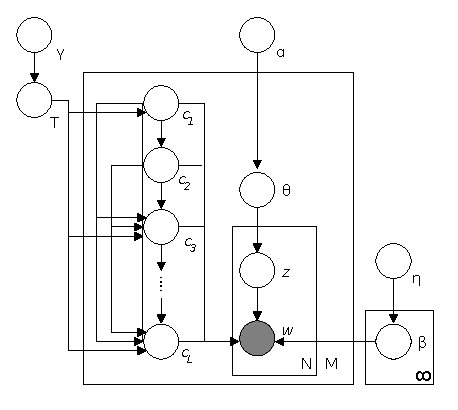
\includegraphics[scale = 0.8]{hLDA_paper.eps}}
				\caption{Illustration of generative process of hLDA \cite{2}}
				\label{fig: hLDA}
			\end{figure}

\subsection*{Dynamic Topic Model (DTM)}
Dynamic topic models (DTM) \cite{3} can be seen as a combination of LDA and time series. It is a generative model that analyzes the time evolution of topics of a collection of documents over time.\newline
The generative process of DTM (Figure~\ref{fig: DTM}) is as follows, where time t is discretized in to time slices:
\begin{enumerate}
  \item Draw topics $\beta_{t} |\beta_{t - 1} \sim N(\beta_{t-1}, \sigma^2I)$.
  \item Draw $\alpha_{t} |\alpha_{t - 1} \sim N(\alpha_{t-1}, \delta^2I)$.
  \item For each document:
  	\begin{enumerate}
  	  	\item Draw $\eta \sim N(\alpha_t, a^2I)$
    		\item For each word:
			\begin{enumerate}
  	  			\item Draw $Z \sim Multinomial(\pi(\theta))$.
    				\item Draw $W_{t,d,n} \sim Multinomial(\pi(\beta_{t,z})$, with $\pi(\beta_{k,t})_w = \frac{exp(\beta_{k,t,w})}{\sum_w exp(\beta_{k,t,w})}$
			\end{enumerate}
  	\end{enumerate}
\end{enumerate}
Here, $\beta$ and $\theta$ are not sampled from Dirichlet distributions as in smoothed LDA, instead, $\beta_{t,k}$ is a random walk with Gaussian steps, while $\theta$ is drawn from a logistic normal with mean $\alpha_t$, which undergoes similar dynamics as $\beta_{t,k}$. The choice of logistic normal is due to its amenability with time series modeling. \newline
DTM computes the posterior of hidden variables of all the time slices, which is used to output the evolution of topics and keywords.
\begin{figure}[!ht]
				\centerline{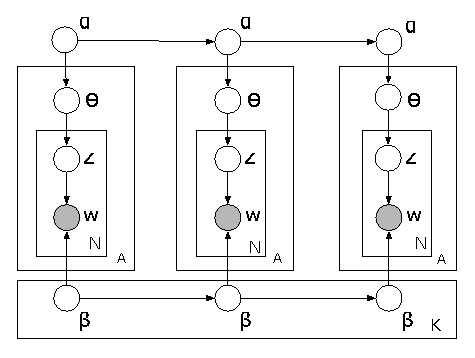
\includegraphics[scale = 0.8]{p113-blei.eps}}
				\caption{Illustration of generative process of DTM \cite{3}}
				\label{fig: DTM}
			\end{figure}

\section*{Data Collection}
\subsection*{Data Source}


\subsection*{Feature Extraction}
The collection of abstracts have to be converted to a term frequency matrix as required by all the topic models described above. Instead of generating a term matrix with raw data, we pre-process the data as follows to remove noise:
\begin{enumerate}
  \item Separate an abstract into sentences.
  \item For each sentence:
    	\begin{enumerate}
  	  	\item Remove stop words (e.g. 'the', 'and', 'of').
		\item Remove tokens containing no letters.
		\item Remove common verbs (e.g. 'get', 'take', 'think').
		\item Remove tokens shorter than minimum term length of 3 characters.
		\item Remove latex format tokens.
		\item Split hyphen connected words if both words are longer than the minimum term length.
		\item Convert nouns to sigular form and verbs to infinitive form.
		\item Stem tokens.
  	\end{enumerate}
\end{enumerate}
Then we generate a dictionary containing all terms that appeared in at least 5 documents and a term matrix whose (i, j)-th element n denotes that the j-th word in the dictionary occurred n times in the i-th document. 
 
\subsection*{Feature Transformation}
While doing data pre-processing, we observed that new concepts in science and technology are usually expressed in the form of phrases, such as "computer science", "machine learining" and "topic modeling", which indicates a topic might be better characterized by its "key phrases" instead of keywords. Furthermore, phrases also offer better interpretability of results, e.g. a topic with keywords {"dimension", "principal", "analysis"} may greatly perplex us, while one with key phrases {"principal component analysis", "dimension reduction"} is quite informative.\newline
We generated phrases before the second step in the previous section by:
\begin{enumerate}
  \item Separate words into blocks by punctuation marks and stop words.
  \item Within each block, generate phrases made up of consecutive words while restricting the maximum length of phrases to 5 words since usually phrases longer than 5 words are represented by their acronyms.
\end{enumerate}

\subsection*{Feature Weighting Schemes}


\section*{Experiments}

\subsection*{Data Collection}
Data is crawled from the online archive website arXiv. In fields like mathematics and physics, almost all scientific papers are self-archived on the arXiv. Despite not peer reviewed, arXiv has its submissions reviewed (or even recategorized if off-topic) by moderators that are experts in their fields of research. In addition, submission dates on arXiv more accurately reflect when the research project was completed and paper drafted, since usually papers are posted on arXiv months before they are finally published on a peer reviewed journal or conference. Based on these facts, we believe arXiv is a better collection of research works than any journal or conference alone.\newline
The titles, authors, abstracts and citation of papers are scraped from API of \url{http://export.arxiv.org/api/} using Python and stored in separate files according to the publish year. We used only papers in condensed matter physics from year 1992 to 2003, but the methods demonstrated in this report can be applied to the analysis any field. The corpus contains 14185 abstracts, 4645 unique words and 11255 unique phrases after data pre-prodessing.


\subsection*{Results}
\subsubsection*{Dynamic Topic Model}
In our DTM experiment, the number of topics is set to 10 a priori. Results are summarized in Figure ~\ref{fig: DTM_table_unweight} and Figure ~\ref{fig: PhaseTrans_wp}. In Figure ~\ref{fig: DTM_table_unweight} we demonstrate 5 out of the 10 topics for purpose of figure size control, the 3 tables respectively are topics and keywords generated from only words, words plus phrases and only phrases. The classification with phrases clearly gives much better interpretability. Note that the first two tables look quite similar, in fact, in the second table, even though the corpus contains both words and phrases, we can hardly see any phrases among the important keywords. This is quite intuitive since in the corpus, there are 486712 words, 4645 of them unique and 112448 phrases with 11250 of them unique. So on average, a word appears ~100 times in the corpus while a phrase appears only ~10 times, resulting in a term matrix dominated by words. This is what has motivated our weighting scheme. \begin{figure}[!ht]
  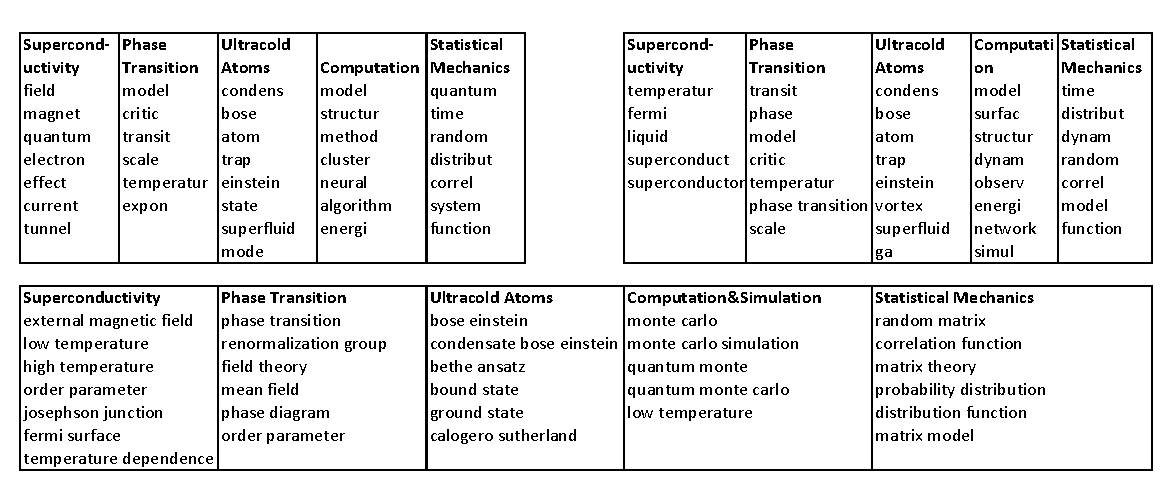
\includegraphics[scale = 0.45]{dtm10_unweight.eps}
  \caption{DTM Topics and Keywords}
  \label{fig: DTM_table_unweight}
\end{figure}
In Figure ~\ref{fig: DTM_table_unweight}, we present the plot of one specific topic "phase transition", which is typical of all the plots.
\begin{figure}[!ht]
  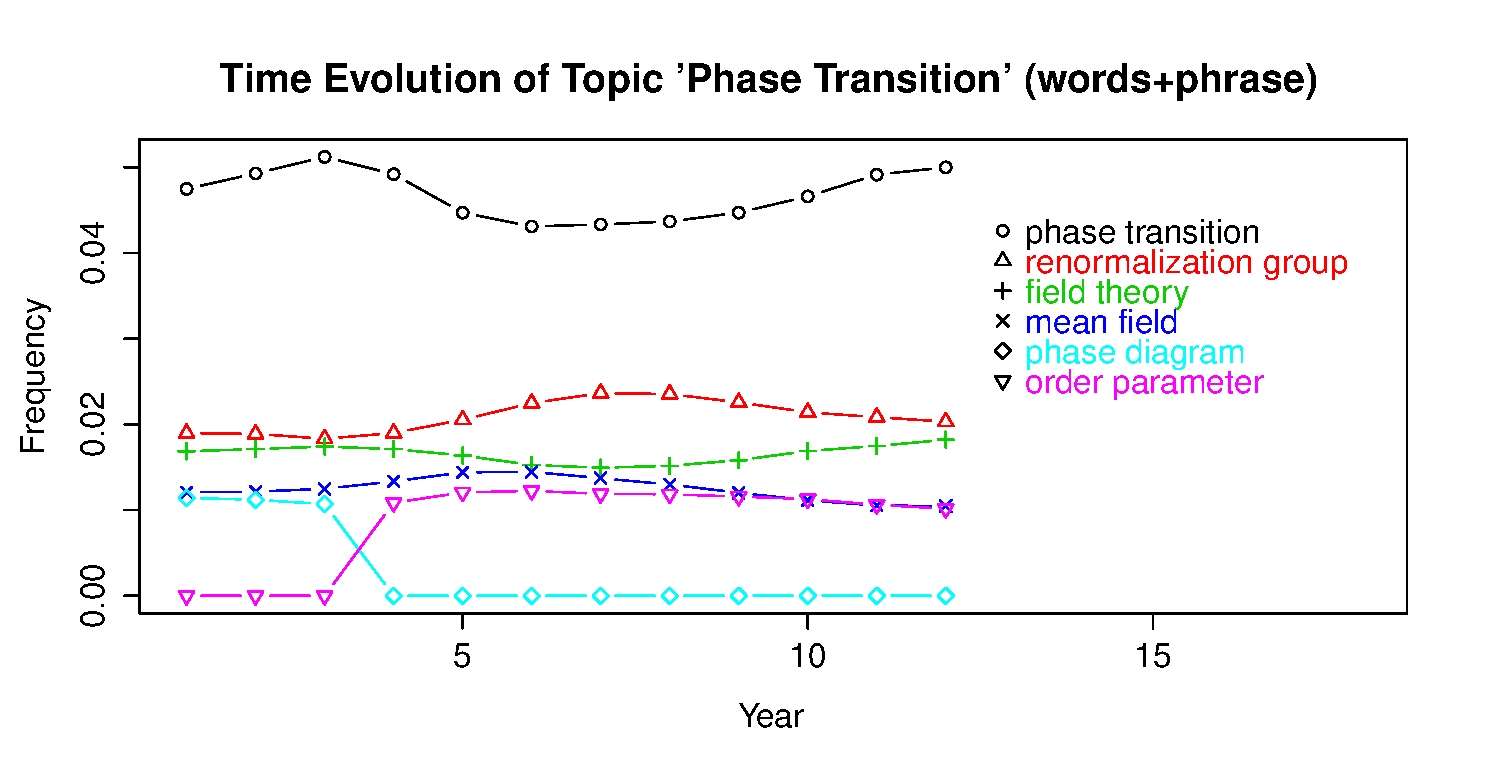
\includegraphics[scale = 0.365]{PhaseTrans(w_p).eps}
  \caption{Keywords Trend Plot of Topic "Phase Transition"}
  \label{fig: PhaseTrans_wp}
\end{figure}[!ht]
From Figure ~\ref{fig: DTM_table_unweight}, despite the frequencies of keywords do rise and fall, there is hardly any obvious "trend". This is not unexpected since it's natural that a paper on "phase transition" should always involve keywords such as "phase transition" and "phase diagram" regardless of when it is published.\newline
One very informative plot we can make is the evolution of topic popularity. In Figure ~\ref{fig: TopPop_p}, we show a plot of frequencies for 4 topics over time.
\begin{figure}[!ht]
  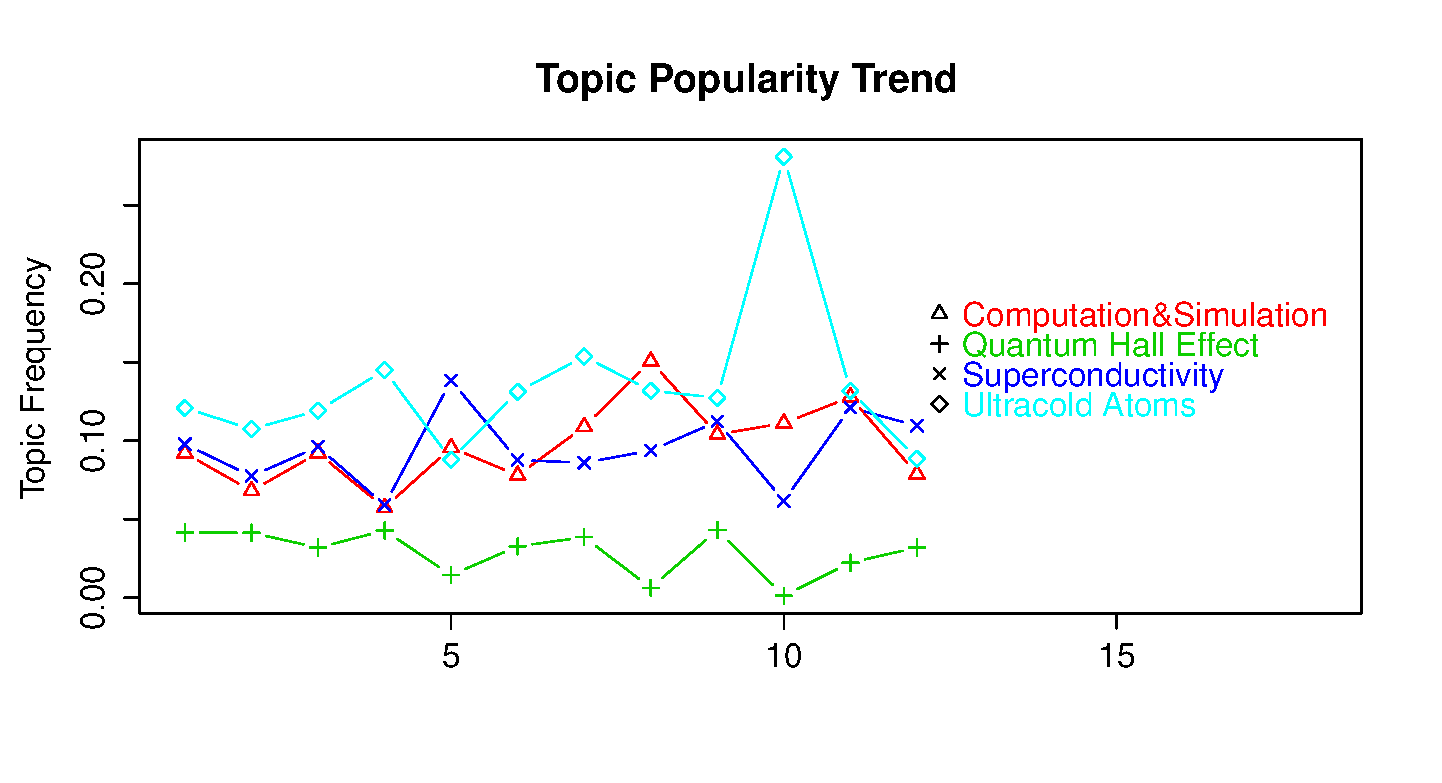
\includegraphics[scale = 0.365]{TopPop_p.eps}
  \caption{Plot of Frequencies of Different Topics over Time}
  \label{fig: TopPop_p}
\end{figure}
This plot has some really interesting implications: 
\begin{inparaenum}[\itshape a\upshape)]
\item "Superconductivity" and "Ultracold Atoms" are clearly negatively correlated, which indicates it is possible that for some reason (e.g. similarities in research techniques) research works in these two fields are almost done by the same group of researchers. The negative correlation is created by the shift of their interest and time allocation between the two fields. So for a Phd student whose thesis project is in superconductivity, it may be wise to choose a backup side project in "Ultracold Atoms", in the case her thesis project fails, she can turn to the side project and produce some results quickly without having to acquire a new set of skills.
\item In certain field, it is easy to publish, but difficult to discover something of importance, while it's the opposite case in some other fields: "Quantum Hall Effect", although being quite famous even outside the field of physics has actually very few publications, which is probably due to the requirement of ultra high magnetic field in quantum Hall experiments. On the other hand, there are surprisingly large number of papers on "Computations and Simulations" despite the small number of researchers in this field (e.g. one out of about 40 physics faculty members at Stanford). This implies that if one's priority is to have as much publication as possible, then he should choose to do simulations.
\end{inparaenum}

\subsubsection*{Hierarchical Latent Dirichlet Allocation}
 We produced three depth 4 trees generated words alone, words plus phrases and phrases alone, where the depth has to be chosen a priori. Branches with less than 30 keywords are pruned off. In Figure 7, we show the ** tree up to the fourth level, while the other two to the third level, because there are already too many branches on the third level. tree generated by words only, we only show the trees only up to the third level  fourth level to limit size of the plot. We also only display the first three branches from each node to limit the size of the tree, there are usually 5 trees from each node.

We used abstracts of the first 6000 submissions to the condensed matter section as our corpus. A term matrix generator (TMG) \cite{5} with stop words filter is used to generate a dictionary containing all terms that appeared in at least 5 documents and a term matrix whose (i, j)-th element n denotes that the j-th word in our dictionary occurred n times in the i-th document. The resulting matrix had 19327 terms and was fed thru an off the shelf C-package "hlda-c" \cite{1} implementing hLDA.\\
A depth 4 tree generated by "hlda-c" looks like:\newline
			\begin{figure}[!ht]
				\centerline{\includegraphics[scale = 0.35]{phrase.png}}
				\caption{Unsupervised Hierarchical Classification of First 10000 Submissions to Condensed Matter Physics Section}
			\end{figure}
\newline
Despite being completely unsupervised, the result is actually surprisingly good. The three numbers in square brackets before each line are tree level, number of terms and number of documents in this branch. The top node (0th - level ) contains the function words. In the next level, the documents are classified into three branches: first class containing 5539 documents, second class containing 417 documents and the third class containing 44 documents. Eventhough the dataset seem to very skewed, with the largest class containing 100 times more documents than the smallest class, the classification captures sub fields in condensed matter physics very nicely: the first class is still very large, so its keywords are still pretty much function words, but if we go a level down to level 2, we can see the first branch contains mostly theoretical studies on correlated systems such as superconductors, antiferromagnet, quantum Hall and Bose Eistein condensation; the second branch contains experimental papers on material growth and transport measurements; Second class on level 1 is topics on studies in the intersection of condensed matter physics and chemistry, namely material synthesis; third branch on level 1 contains topics on computational physics -- using computational methods to calculate physical and chemical properties of materials. The hierarchical clustering not only gives us a very good idea what the sub fields are, but also ranked them according to their popularity, which agrees well with our knowledge of the field.      

\section*{Discussion}

\section*{Acknowlegement}
We would like to thank the TAs for their guidance and advice for this project. We also want to thank Prof. Andrew Ng for introducing us to the exciting field of machine learning.  
%----------------------------------------------------------------------------------------
%	REFERENCE LIST
%----------------------------------------------------------------------------------------

\begin{thebibliography}{99}

\bibitem[1] {1}
  Blei, D., Ng, A. and Jordan M.
  \emph{Latent Dirichlet Allocation}.
  The Journal of Machine Learning Research,
 Volume 3, 993 - 1022
 Mar 2003
 
\bibitem[2] {2}
  Blei, D., Griffiths, T. and Jordan M.
  \emph{Hierarchical Topic Models and the Nested Chinese Restaurant Process}.
  NIPS,
 2003.
 
 \bibitem[3] {3}
  Blei, D., Griffiths, T., Jordan M., and Tenenbaum J. 
  \emph{Dynamic Topic Models}.
  Proceedings of the 23rd International Conference of Machine Learning ,
 Pittsburgh, PA,
 2006
 
 \bibitem[4] {4}
  Blei, D. and McAuliffe, J.
  \emph{Supervised Topic Models}.
 
 \bibitem[5] {5}
  D. Zeimpekis and E. Gallopoulos
  \emph{TMG: A MATLAB-based term-document Matrix Constructor for Text Collections}.
  Technical Report, Computer Engineering and Information Department, University of Patras
  Dec 2003
  http://scgroup20.ceid.upatras.gr:8000/tmg/

\end{thebibliography}
%----------------------------------------------------------------------------------------

\end{document}